%% Lee
%% In dissertation, change 
%    section* to chapter 
%    subsection* to section
%    subsubsection* to subsection

% >>>>>>>>>>>>>>>>>>>>>>>>>>>>>>>>>>>>>>>>>>>>>>>>>>>>>>>>>>>>>>>>>>>>>>>>>>>>> DRAM Customizable <<<<<<<<<>>>>>>>>>>>>>>>>>>>>>>>>>>>>>>>>>>>>>>>>>>>>>>>>>><<<<<<<<<<<<<
%\chapter{DRAM Overview and Customizations}
\section{DRAM Overview and Customizations}
\label{sec:DRAM Customizations}

There are two types of memory employed in \acp{asic} and \acp{asip}, \acf{sram} and \acf{dram}.
Both of these technologies have a similar top-level block diagram which contains an array of storage elements, a means to address into a particular row of memory cells and a means to read and write a column of those cells.
A basic block diagram is shown in Figure \ref{fig:MemoryBlockDiagram}.
%\begin{figure}[!t]
\begin{figure}[h]
% the [] contains position info e.g. [!t] means here
\centering
\captionsetup{justification=centering}
\centerline{
\mbox{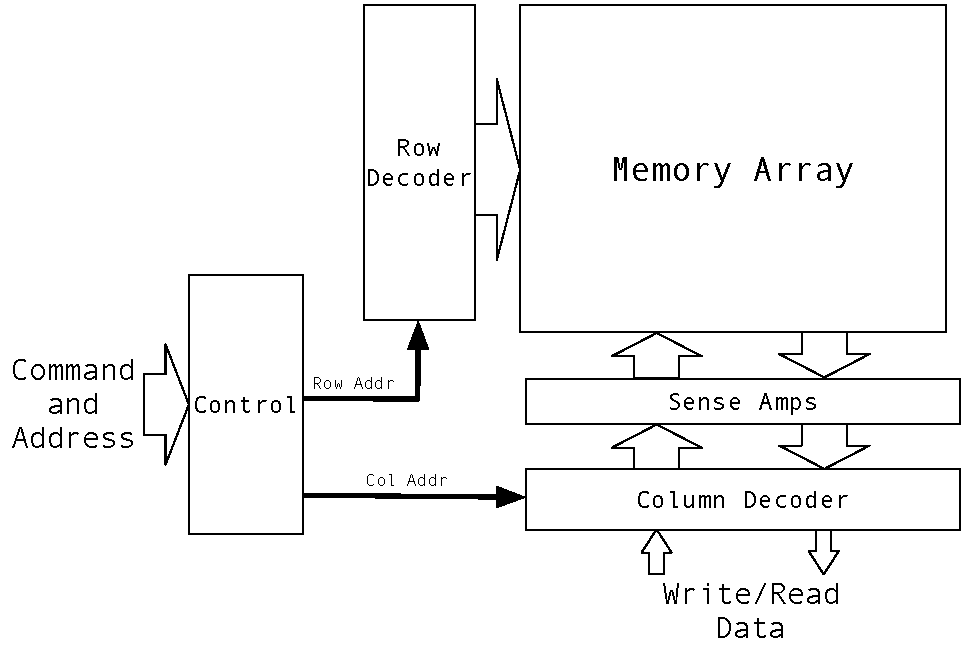
\includegraphics[width=.8\linewidth]{BasicMemoryBlockDiagram}}
}
\caption{Typical Memory Block Diagram \cite{Jacob:2007:MSC:1543376}}
\label{fig:MemoryBlockDiagram}
\end{figure}


\begin{figure}[h]
\centering
\begin{subfigure}{.45\textwidth}
  \centering
  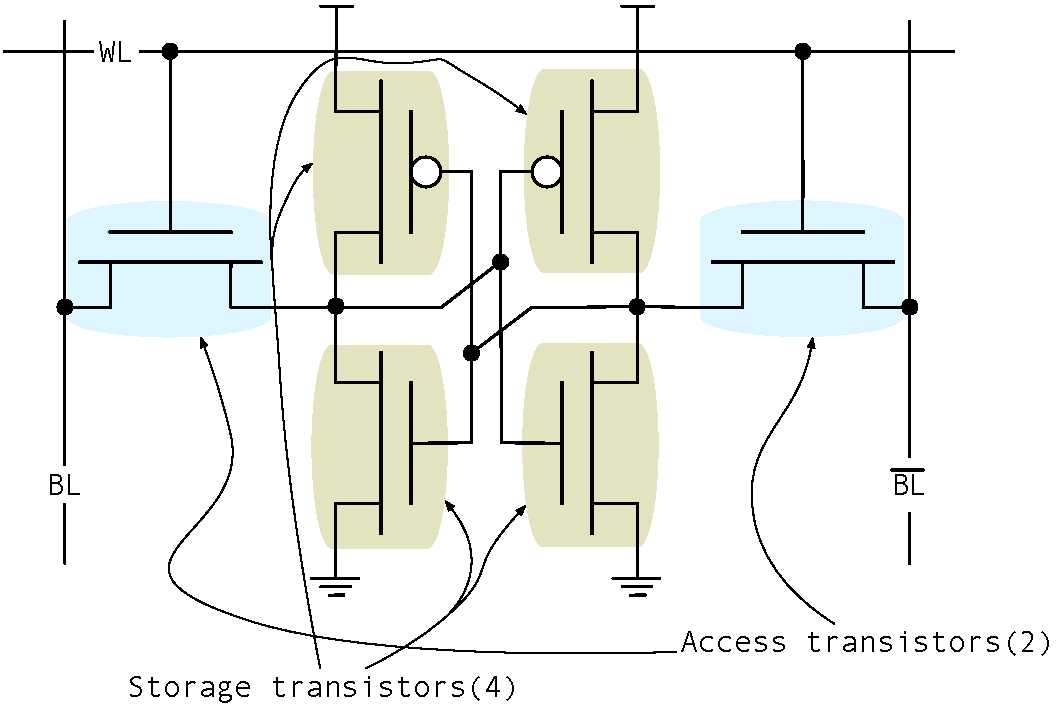
\includegraphics[scale=0.4]{SRAM_Cell}
  \captionsetup{justification=centering, skip=5pt}
  \vspace{-6pt}
  \caption{SRAM Storage Cell \cite{Jacob:2007:MSC:1543376}}
  \label{fig:SRAM Cell}
\end{subfigure}%
\begin{subfigure}{.45\textwidth}
  \centering
  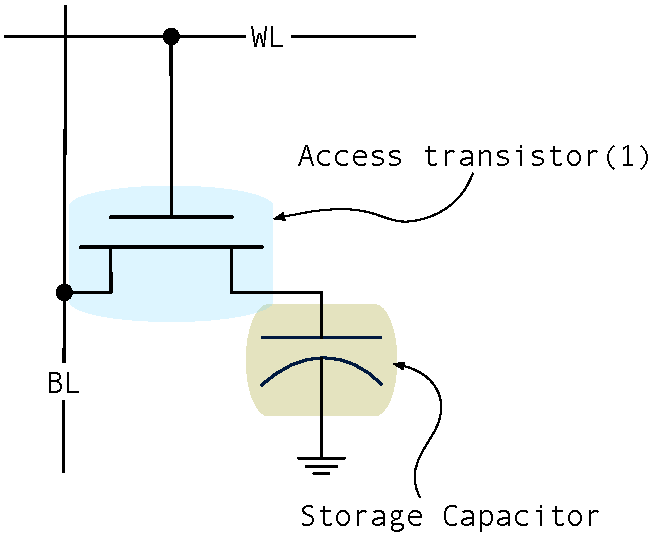
\includegraphics[scale=0.4]{DRAM_Cell}
  \captionsetup{justification=centering, skip=5pt}
  %\vspace{36pt}
  \vspace{20pt}
  \caption{DRAM Storage Cell \cite{Jacob:2007:MSC:1543376}}
  \label{fig:DRAM Cell}
\end{subfigure}
\captionsetup{justification=centering, skip=12pt}
\caption{RAM Storage Cell Types}
\label{fig:Memory Storage Cells}
\end{figure}

\iffalse The major difference between the \ac{sram} cell and \ac{dram} cell is the number of elements it takes to implement. \fi
The \ac{sram} cell takes six transistors (figure \ref{fig:SRAM Cell}) and the \ac{dram} cell takes one transistor and one capacitor (figure \ref{fig:DRAM Cell}).
This means the \ac{dram} arrays provide five to six times more storage density when compared to a similar sized \ac{sram} array.

The major disadvantage is the capacitor cannot hold a charge indefinitely because the leakage currents in \acp{ic} cause the charge to leak away. 
If kept unchecked, the stored value will dissipate and it is this behavior that makes accessing a \ac{dram} array more complicated than a similar \ac{sram} array.

\subsection{Accessing \ac{dram} and \ac{sram}}
\label{Accessing DRAM and SRAM}

Accessing a typical \ac{sram} involves providing an address and either reading or writing the contents of that location. 
The read or write often completes in one or two clock cycles depending on whether the \ac{sram} employs internal registers which are used run the \ac{sram} with a faster clock.
The storage cell inside the \ac{sram} is formed from cross-coupled transistors (see Figure \ref{fig:SRAM Cell}) which latch the contents and hold the contents indefinitely or until power is removed from the device.
The storage structure employs six transistors and allows the access logic to be relatively simple and fast but has a relatively low density because of the number of transistors employed.

Accessing a ``typical'' \ac{dram} is much more involved. It involves opening a page in a bank, reading or writing a portion of the contents of the page then closing the page. 
%When an \ac{sram} cell is read, the cross-coupled transistors retain the stored value. 
The reasons behind this added complexity is the memory cell inside the \ac{dram} which is formed from a capacitor (see Figure \ref{fig:DRAM Cell}) which holds a charge reflecting a logic zero or one. 
When a page(row) of a \ac{dram} memory array is read by the sense amps (see Figure \ref{fig:dramBlockDiagram}), the process of sensing the charge on the capacitor causes the capacitor to discharge and lose its contents. 
To alleviate this problem \iffalse \ac{dram} arrays are formed from a column of storage elements known as a page. \fi when the read occurs, the entire contents of the page are transferred to registers, referred to as ``page intermediate store'' in Figure \ref{fig:dramBlockDiagram}. 
The process of transferring a page to the intermediate store is known as a ``page open''.
Once this transfer is complete, portions of the open page can be read similar to reading an \ac{sram}. 
The problem is that if another read wants to access data that is not in the page, the page has to be closed and another page opened. 
This involves transferring the previously registered page back to the array to recharge the capacitors in the memory array storage elements. 
The next page can then be opened and transferred to the page intermediate registers.

In practice, the \ac{dram} protocol is separated into ``page'' commands and ``cache'' commands. The page commands open and close pages and the cache commands read and write to the page intermediate store.
The process of opening and closing pages is a relatively long time, typically 10-20\SI[per-mode=symbol]{}{\nano\second}. Once a page is open, accessing the intermediate store is much faster.
So if the accesses are somewhat random and different pages are constantly accessed and pages are constantly being opened and closed, the average time to complete reads and writes are very large when compared to \ac{sram}.
To alleviate this issue, the \ac{dram} is formed from more than one array of storage elements, between 8 and 32, known as banks. The idea is that while a page from one bank is being accessed, another banks page can be opened in preparation for a future read (or write).
This access protocol is rather complicated and involves interleaving page commands and cache commands to multiple banks. 
The system memory controller logic must keep track of which pages are open inside the \ac{dram} and for each memory request must determine if a page needs to be closed and another opened before reading (or writing) the intermediate store.
If consecutive accesses are not sequenced carefully, the performance of \ac{dram} can be poor.

Some key characteristics of the \ac{dram} used in this work can be seen in Table \ref{tab:DiRAM4 characteristics}. 


\subsubsection{Access Locality/Reuse and \ac{sram} as a Cache}
\label{Access Locality/Reuse and Cache}

In general purpose computing, the sequence of accesses cannot always be controlled, so \ac{sram} is typically used as the first level of memory with \ac{dram} used as the primary storage. 
Using \ac{sram} as this first level memory is called a cache and acts like a mirror of the \ac{dram} contents.
These caches have been used for decades to isolate the computing system from unpredictable access behavior of the \ac{dram}.
The general idea behind caches is that most data exhibits spatial and temporal locality. This ``locality'' means that when a computer program uses a piece of data in memory, it is very likely that soon after other data ``close'' to that data will be used and/or the same data will be reused.
So when a piece of data in memory is accessed, that data and a large block of data in close proximity to the requested data are transferred to the cache. 
The cache is designed to hold multiple of these blocks of data often resulting in tens of \SI[per-mode=symbol]{}{\kilo \byte} of \ac{sram}.
When other memory requests are made, the memory controller checks to see whether the block associated with the requested data is present in the cache.
If the requested data is contained in a block present in the cache, this is considered a ``hit'' and the data in the cache is used. 
If the requested data's block is not present, this is known as a ``miss'' and the slower main memory must be accessed. This access results in another ``block'' of data being transferred to the cache.
If all the blocks in the cache are currently fully employed, one of the blocks must be freed up to make space in the cache for the new block. 
A block is chosen and transferred back to the main memory and the new block is read and transferred to the cache.
To make effective use of the cache, the access behavior of the computer program must exhibit this locality behavior. 
If the cache blocks are large enough and the program's access behavior exhibits locality, then employing \ac{sram} is effective and the slower \ac{dram} access times can be somewhat hidden.

As mentioned in Section \ref{sec:overview} much of the \ac{asic} and \ac{asip} \ac{ann} research has focused on taking advantage of the performance and ease of use of \ac{sram}. 
If the target application's memory access behavior exhibits some locality and the \ac{sram} cache can be made large enough to avoid high levels of cache misses, then this use of \ac{sram} can be effective.
But this work's target application is such that the access behavior exhibits no or little locality (reuse) and block transfers between the cache and main memory would be constantly occurring.
Under these circumstances, \textbf{\textcolor{black}{\ac{dram} bandwidth will be the bottleneck}}.

This work focuses on using \ac{dram} as the primary storage and managing the accesses to ensure the \ac{dram} is used effectively. 
With the increased bandwidth achieved from the additional \ac{dram} customizations discussed in Section \ref{sec:Very-Wide Bus} and \ref{sec:Write Mask}, this work demonstrates \ac{dram} bandwidths 10X faster than what is available with 2 or 2.5D solutions.
This high level of \ac{dram} bandwidth provides this work the ability to process multiple disparate \acp{ann} at or near real-time while being \textbf{\textcolor{black}{significantly faster than state-of-the-art solutions}}.


\subsection{DRAM Customizations}

In a typical \ac{dram}, a bank may contain on the order of a few thousand pages and a page may contain on the order of a few thousand bits.
Once the page is open, the user accesses a portion of the requested page over a bus. With PCB based DRAMs the bus might vary from four to 16 bits wide, but with 3D DRAMs, such as HBM the bus might be up to 128 bits wide.
An \ac{asic}, \ac{asip} or \ac{gpu} implementation may combine multiple devices to generate bus widths on the order of \SI[per-mode=symbol]{1}{\kilo \bit} wide. 
When using 2.5D technology and \ac{hbm} with their Pascal\texttrademark \ac{gpu} accelerator device, NVidia\textregistered ~achieve a raw \ac{dram} bandwidth approaching \SI[per-mode=symbol]{6}{\tera \bit \per \second} \cite{Nvidia_p100_summary_datasheet}\footnote{datasheet also shows a \ac{tdp} of \SI[per-mode=symbol]{300}{\watt}}.
However, experience has shown \cite{farabet2011neuflow} \cite{jouppi2017datacenter} that usable bandwidth will likely be much lower.
Regardless, this existing technology does not achieve the required bandwidth \eqref{eq:maximumBandwidth}.


%Considering systems will want to perform multiple \ac{dnn}s simultaneously suggests that these embedded systems will require usable memory bandwidth of the order of 10s of \SI[per-mode=symbol]{}{\tera \bit \per \second} \eqref{eq:maximumBandwidth}.

To achieve increased \ac{dram} bandwidth this work is proposing two changes to the Tezzaron\textregistered \ac{diram4} \cite{tezzaron:diram4} \ac{3d} \ac{dram}. 
The most significant customization is to widen the databuses to generate more raw bandwidth. This is discussed further in Section \ref{sec:Very-Wide Bus}.
With the customizations discussed in Sections \ref{sec:Very-Wide Bus} and \ref{sec:Write Mask}, this work demonstrates \ac{dram} bandwidths >10X faster than what is available with 2 or 2.5D solutions.

\subsubsection{Customization One: Very-Wide Bus}
\label{sec:Very-Wide Bus}

This work achieves the increase in bandwidth by proposing that the DRAM expose more of its currently open page. This means providing access to larger portions of the ``Page intermediate store'' shown in Figure \ref{fig:dramBlockDiagram}.
Without the limitations of having to transfer data beyond the chip stack, this work suggests exposing a larger portion of the page over a very wide bus. 
By staying within the 3D footprint, this bus can be implemented using fine pitch \acp{tsv} (see Figure \ref{fig:dramBusChange}).
This work assumes the \ac{dram} interface protocol uses \ac{ddr} with a bus width of 2048. Given the \ac{diram4} employs a burst of two for read and write cycles, an entire \ac{diram4} page of 4096-bits is accessed during each read or write. 
\begin{figure}[!t]
% the [] contains position info e.g. [!t] means here
\centering
\captionsetup{justification=centering}
\centerline{
\mbox{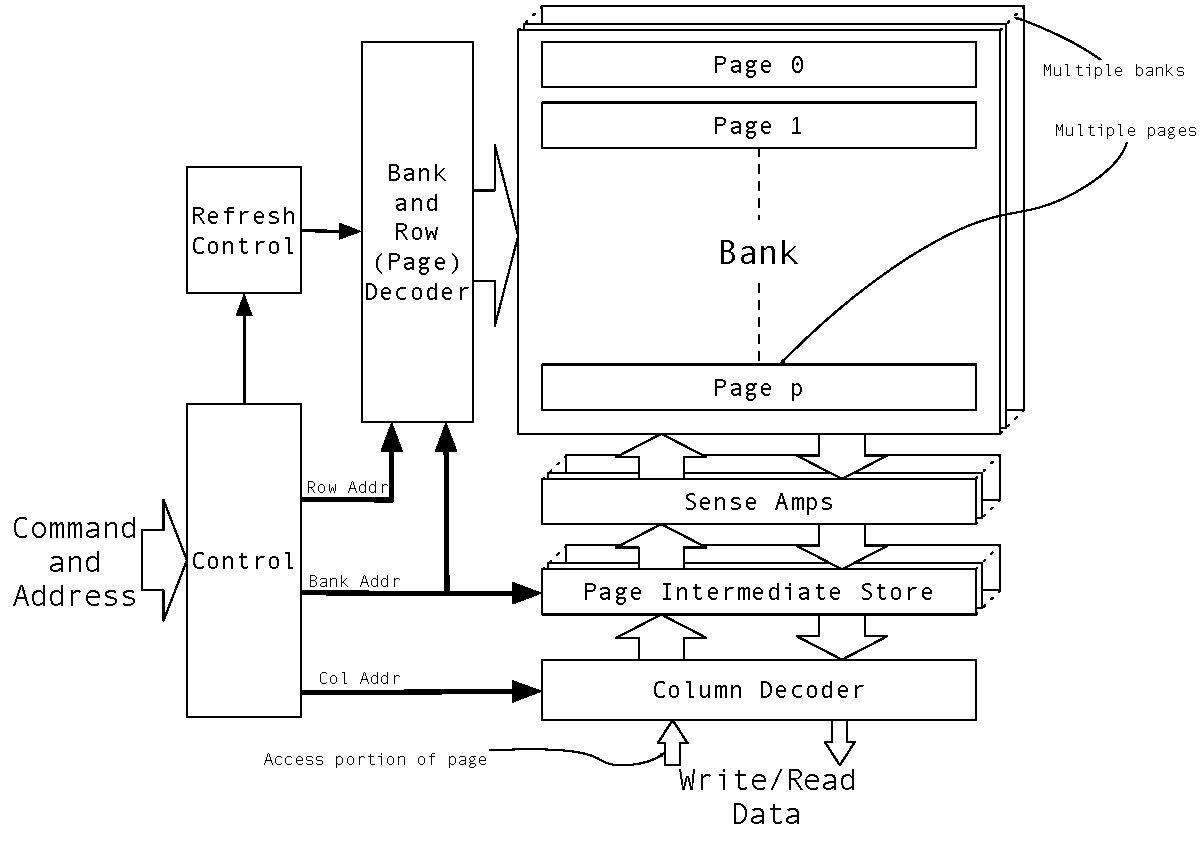
\includegraphics[width=.75\linewidth]{DRAMBlockDiagram}}
}
\caption{Typical DRAM Block Diagram \cite{micron_ddr3}}
\label{fig:dramBlockDiagram}
\end{figure}

\begin{figure}[!t]
% the [] contains position info e.g. [!t] means here
\centering
\captionsetup{justification=centering}
\captionsetup{width=.75\linewidth}
\centerline{
\mbox{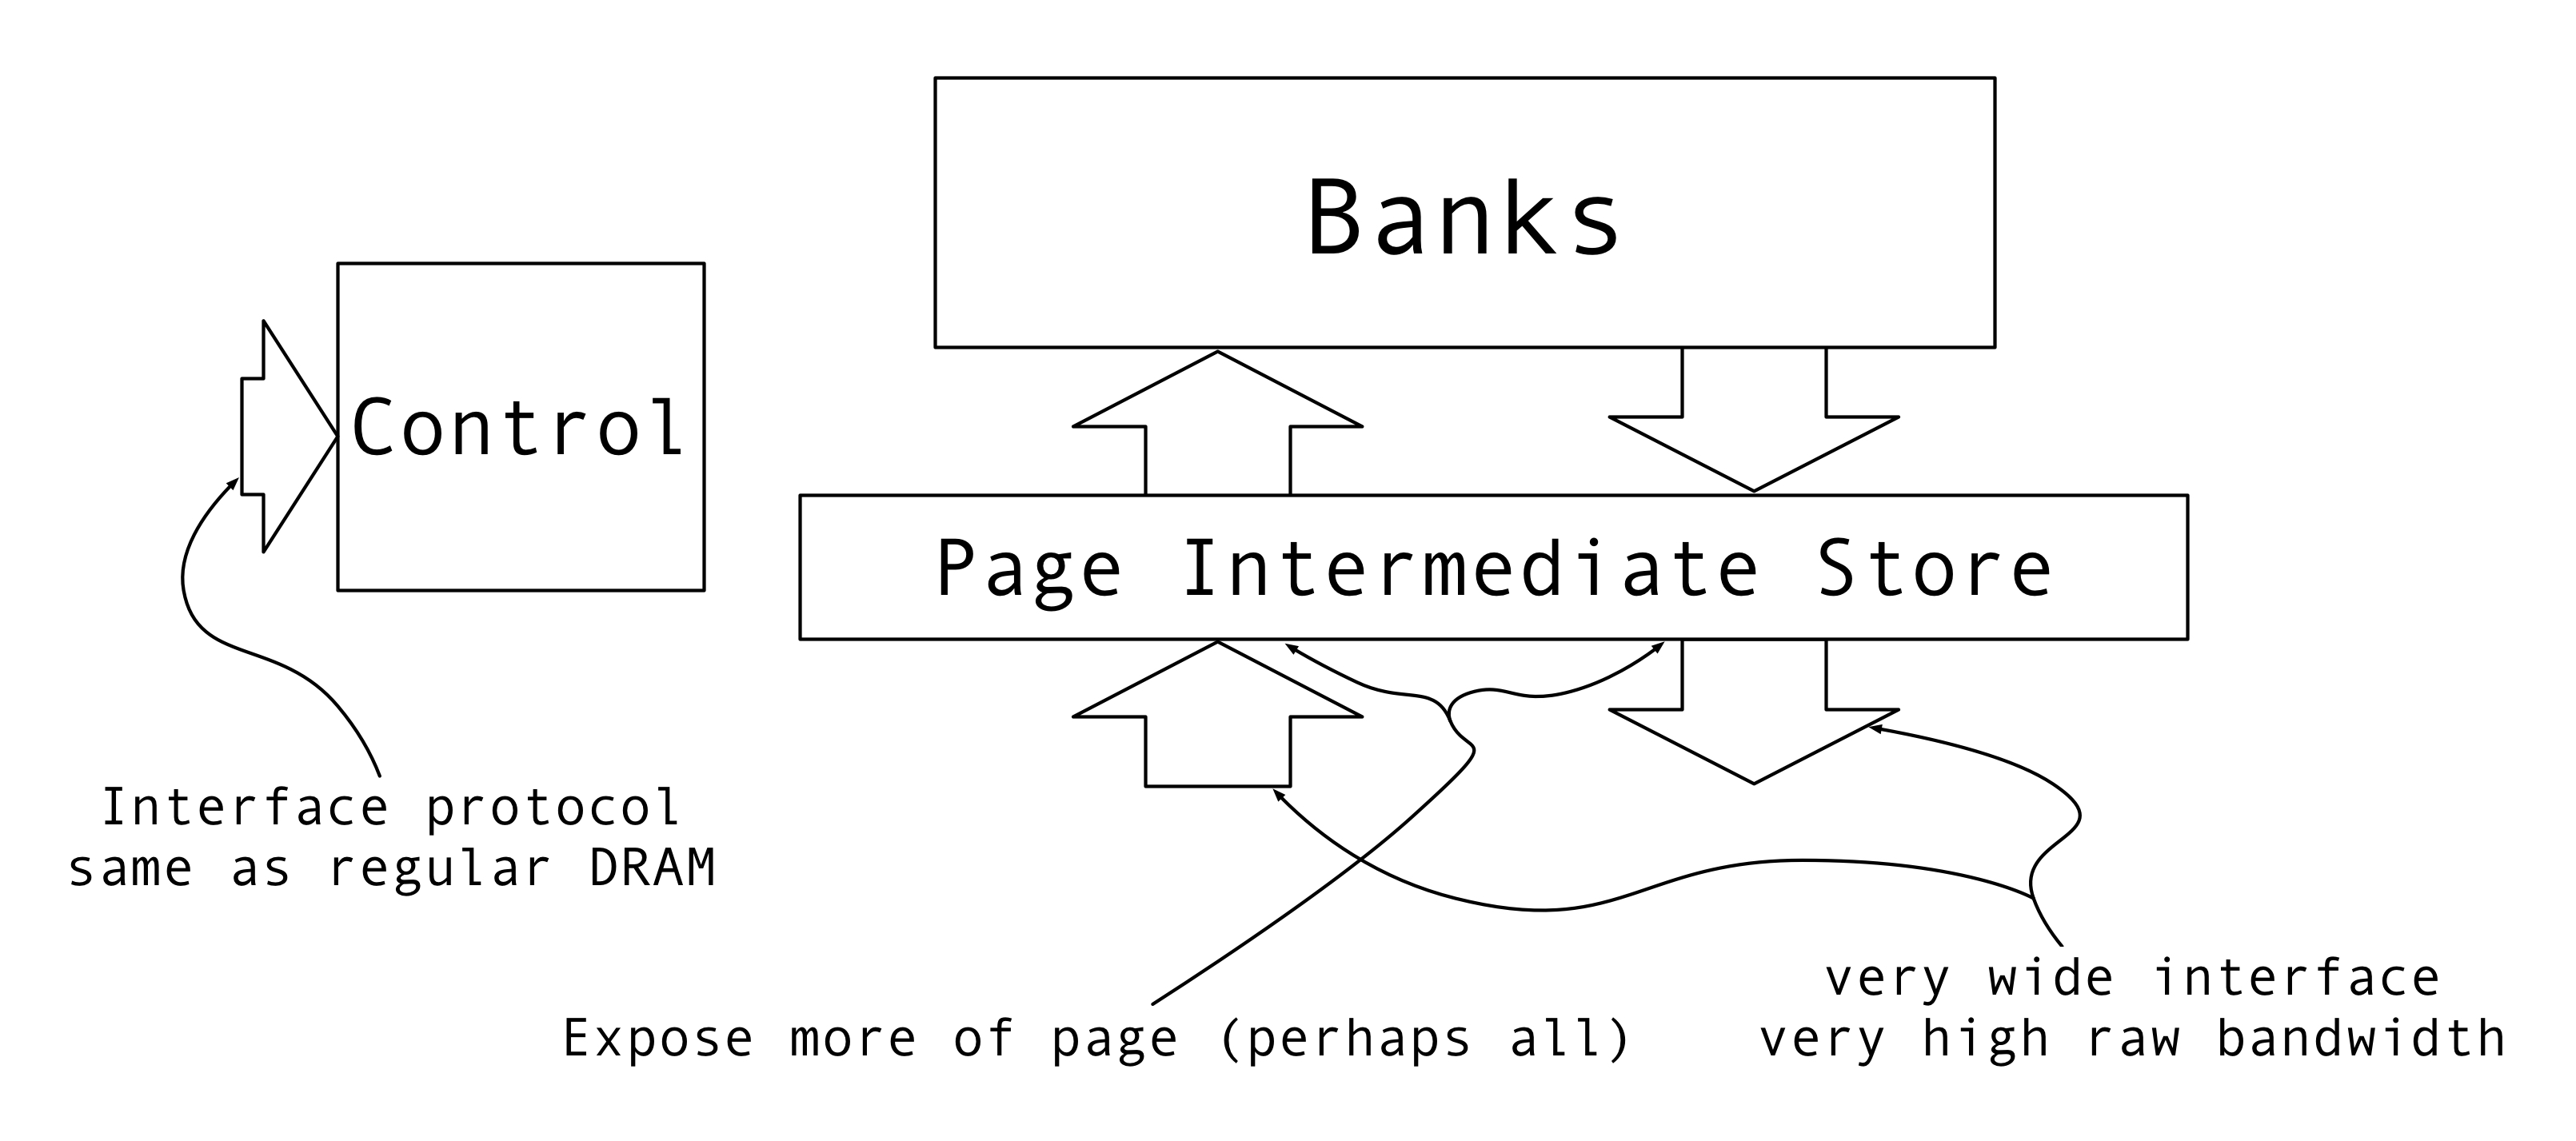
\includegraphics[width=.65\linewidth]{DRAMBusChange}}
}
\caption{Exposing more of the DRAM page}
\label{fig:dramBusChange}
\end{figure}

\subsubsection{Customization Two: Write Mask}
\label{sec:Write Mask}
When processing an \ac{ann}, to compute the activation of an individual \ac{an} involves reading the pre-synaptic \ac{an} activations and the weights of the connections between the pre-synaptic \acp{an} and the \ac{an} being processed. 
Typically, a group of up to 32 \acp{an} are processed. Assuming the state of an \ac{an} is represented by a \ac{binary32} number format, the memory used to store the states of the group of \acp{an} represents only up to 25 percent of a \ac{dram} page.
If a partial page needs to be written, the write controller with have to read the page, then modify the page with the new data and write the modified page back to memory.
To minimize writing partial pages, the write controller has temporary registers to store two pages of data. 
The write controller accumulates the \ac{an} states in these temporary registers before writing back to memory.
If the write controller receives any data that is not destined for the pages associated with the temporary registers, the contents of one of these page registers must be written back to memory to accomodate the new data.
If the register chosen to be written back to memory only contains a partial page of data, the write controller would need to perform a read/modify/write operation.
The ratio of reads to writes is high, hundreds or thousands to one so this additional read/modify/write will not adversly affect the performance. 
However, a proposed customization to the DRAM is the addition of a write data mask to the \ac{dram} write path thus avoiding this read/modify/write.
This work assumes single precision floating point for \ac{ann} weights and activation, so a mask bit will be provided on a word basis or every 32 bits.

